\documentclass[twocolumn, 12pt]{article}
\usepackage[utf8]{inputenc}
\usepackage{amsmath}
\usepackage{marvosym}
\usepackage{textcomp}
\usepackage{geometry}
\usepackage{array}
\usepackage{wrapfig}
\usepackage{multirow}
\usepackage{graphicx}
\usepackage{float}
\usepackage{wrapfig}
\usepackage{caption}
\usepackage{amssymb}
\usepackage{ulem}

\geometry{a4paper, margin=.75in}



\begin{document}
\small{
%\pagestyle{empty}

\section*{Fluid Mechanics}
%\subsection*{Equations}

\begin{equation*}
    \rho \triangleq \frac{\Delta m}{\Delta \text{\sout{V}}} \hspace{15pt}   SG \triangleq \frac{\rho}{\rho_{H2O}} \hspace{15pt}  \rho_{H2O} = 1000 [kg/m^3]
\end{equation*}

\begin{equation*}
    \gamma \triangleq \rho g    \hspace{15pt}  \mu \hspace{5pt}[kg/m\cdot s] \hspace{15pt}  \nu = \frac{\mu}{\rho}\hspace{5pt}  \text{(kiNUmatic)}[m^2/s]  
\end{equation*}
\begin{equation*}
    \dot{V}=\textbf{u}A \hspace{10pt} P = \dot{V}\gamma h_p \hspace{10pt} \dot{m}=\rho \textbf{u} A \hspace{10pt} \textbf{F}_P = -\int_A PdA
\end{equation*} 

\begin{align*}
    &\text{Newtonian:} & \tau = \mu \frac{\delta u}{\delta y} \hspace{10pt}   \text{or}   \hspace{10pt} \tau = \nu \frac{\delta u}{\delta y}\\
    &\text{Non-Newtonian:} & \tau \alpha \frac{\delta u }{\delta y}
\end{align*}


\subsection*{Flow Visualizations}

\underline{Streamline}:
\begin{equation*}
    \vec{\nabla} \times \textbf{u}=0 \hspace{10pt} \overbrace{\implies}^{z=0} \hspace{10pt}\frac{\delta y}{\delta x} = \frac{v}{u}
\end{equation*}

\noindent
\underline{Pathline}:
\[
\begin{cases}
    x = x_p(t),   \hspace{30pt}& \frac{\delta x_p}{\delta t} = u(\textbf{x},t)\\
    y = y_p(t),                &  \frac{\delta y_p}{\delta t} = v(\textbf{y},t)\\
\end{cases}
\]
\noindent
\underline{Streakline}:\newline
Shows the history of the flow. Start at \(t=0\) and work it out step by step.

\subsection*{Hydrostatics}
\begin{equation*}
    d\textbf{F}_p = \vec{\nabla}(dxdydz)
\end{equation*}
\begin{equation*}
    -\vec{\nabla} +\rho \textbf{g} =0 \hspace{10pt} \implies  \hspace{10pt} \frac{\delta P}{\delta z} = -\rho g
\end{equation*}
\begin{equation*}
    P_{\text{bottom}} = P_{\text{top}} + \sum_{\text{down}} \gamma_i h_i - \sum_{\text{up}} \gamma_j h_j 
\end{equation*}
\begin{equation*}
    P(z) = P_0 \left[ \frac{T_0 - \alpha (z-z_0)}{T_0}  \right]^{g/ \alpha R}
\end{equation*}



\subsection*{Submerged Gate Procedure}
\begin{enumerate}
    \item Determine \(h_c\) from surface of fluid \(\parallel  \vec{g}\)
    \item Calculate \(P_c\)
        \begin{equation*}
            P_c = \rho g h_c
        \end{equation*}
    \item Determine \(\textbf{F}_R\) acting on the gate where \(y_{cp} \bot \vec{y}\)
        \begin{equation*}
            \textbf{F}_R = P_cA_{\text{gate}}
        \end{equation*}
        \item Determine \(y_c\) along \(\vec{y}\)
        \item Determine \(y_{cp}\) along \(\vec{y}\)
            \begin{equation*}
                y_{cp} = y_c + \frac{\Bar{I}}{y_cA_{\text{gate}}}
            \end{equation*}
        \item Sum torques in a useful way
            \begin{equation*}
                \Sigma \tau_{\text{useful location}} =0
            \end{equation*}
\end{enumerate}


\subsection*{Reynold's Transport Theorem}
\begin{equation*}
    \frac{dB_{sys}}{dt} = \frac{\partial}{\partial t} \int_{CV} b\rho dV + \int_{CS}b\rho (\textbf{u}\cdot d\textbf{A})
\end{equation*}


\begin{equation*}
    \frac{dM_{sys}}{dt} =0= \frac{\partial}{\partial t} \int_{CV} \rho dV + \int_{CS}\rho (\textbf{u}\cdot d\textbf{A})
\end{equation*}


\begin{equation*}
    \frac{d\textbf{p}_{sys}}{dt} = \Sigma \textbf{F} =\frac{\partial}{\partial t} \int_{CV} \textbf{u}\rho dV + \int_{CS}\textbf{u}\rho (\textbf{u}\cdot d\textbf{A})
\end{equation*}


\begin{equation*}
    \frac{d\textbf{H}_{sys}}{dt} =\Sigma \textbf{M} = \frac{\partial}{\partial t} \int_{CV} (\textbf{r}\times \textbf{u})\rho dV + \int_{CS}(\textbf{r}\times \textbf{u})\rho (\textbf{u}\cdot d\textbf{A})
\end{equation*}

\subsection*{Euler's Equation}
\begin{equation*}
    -\frac{\partial}{\partial l}(P + \gamma z) = \rho \left(\frac{\partial \textbf{u}_l}{\partial t} + \textbf{u}_l\frac{\partial \textbf{u}_l}{\partial x_l}\right) = \rho \textbf{a}_l
\end{equation*}

{\footnotesize
\begin{itemize}
    \item Incompressible
    \item Fluid accelerates in direction of decreasing piezometric head
\end{itemize}
}

\subsection*{Bernouli's Equations}
\begin{equation*}
    \frac{P}{\gamma} + z + \frac{u^2}{2g}=const. \hspace{12pt} \text{OR} \hspace{12pt} \frac{P}{\gamma} + z -\frac{\omega^2r^2}{2g} = const.
\end{equation*}

{\footnotesize
\begin{itemize}
    \item Steady flow OR Solid body rotation
    \item Incompressible
    \item Applied on a streamline
\end{itemize}
}


%
\subsection*{Energy Equation}
\begin{equation*}
    \left(\frac{P_1}{\gamma}+\alpha_1\frac{\Bar{u}^2_1}{2g}+z_1\right) +h_p = \left(\frac{P_2}{\gamma}+\alpha_2\frac{\Bar{u}^2_2}{2g}+z_2\right) +h_L + h_t
\end{equation*}

\begin{equation*}
    \alpha \triangleq \frac{\int_A \rho \frac{u^3}{2}dA}{\rho \frac{\Bar{u}^3}{2}A} \hspace{10pt} \implies \hspace{10pt} \alpha = \frac{1}{A}\int_A \left(\frac{u}{\Bar{u}}\right)^3dA
\end{equation*}


\begin{equation*}
    \alpha = 1 (\text{uniform}) \hspace{7pt} \alpha = 2 (\text{parabolic}) \hspace{7pt} \alpha \approx 1 (\text{turbulent})
\end{equation*}


\subsection*{Grade Lines}
\begin{equation*}
    EGL = \alpha \frac{\Bar{u}^2}{2g} +\frac{P}{\gamma} +z \hspace{20pt}   HGL = \frac{P}{\gamma} +z
\end{equation*}




%
\subsection*{Head Loss and Friction}
\begin{equation*}
 h_L = f \left(\frac{L}{D}\right)\frac{\Bar{u}^2}{2g} \hspace{15pt} f_{\text{laminar}} = \frac{64}{Re_D}
\end{equation*}

\begin{equation*}
    f \implies \text{look at Moody diagram}
\end{equation*}

\subsubsection*{Colebrook Equation}
\begin{equation*}
    \frac{1}{\sqrt{f}} = -2log_{10} \left( \frac{e/D}{3.7} + \frac{2.51}{Re^{0.9}}\right)
\end{equation*}

\subsubsection*{Swamee and Jain Equation}
\begin{equation*}
    f  = \frac{0.25}{\left[ \frac{e}{3.7D} +\frac{5.74}{Re^{0.9}} \right]^2}
\end{equation*}


%
\subsection*{Dimensionless Terms}
\begin{equation*}
    Re = \frac{\text{inertia forces}}{\text{viscous forces}} = \rho \frac{uD}{\mu} = \frac{uD}{\nu}
\end{equation*}

\begin{equation*}
    Eu = \frac{\text{pressure forces}}{\text{inertia forces}}= \frac{\Delta P}{\frac{1}{2}\rho u^2}
\end{equation*}

\begin{equation*}
    Fr = \frac{u}{\sqrt{gl}}  \hspace{17pt} Ma = \frac{u}{c_{\text{sound}}} \hspace{17pt}  C_D=\frac{\textbf{F}_D}{\frac{1}{2}\rho u^2A}
\end{equation*}



%
\subsection*{Flow Similarity}
\begin{enumerate}
    \item Geometric Similarity (scale model)
    \item Kinematic Similarity (streamlines/velocity field match)
    \item Dynamic Similarity (non-dimensional terms are equal)
\end{enumerate}

\subsection*{Boundary Layers}
\begin{equation*}
    \delta \hspace{5pt} @ \hspace{5pt} u=0.99u_0   \hspace{15pt} \delta^* = \int_0^\delta \left( 1-\frac{u(y)}{u_0} \right)dy
\end{equation*}

\begin{equation*}
    \theta = \int_0^\delta \frac{u(y)}{u_0}\left( 1 - \frac{u(y)}{u_0} \right)dy
\end{equation*}


\subsubsection*{Laminar BL}
\begin{equation*}
    \delta =\frac{5x}{\sqrt{Re_x}} \hspace{15pt} C_f = \frac{0.32}{Re_L^{1/7}}
\end{equation*}

\begin{equation*}
    \tau_{\text{wall}} = \mu \left\frac{\partial u}{\partial y}\right|_{y=0} = 0.332\mu \frac{u_0}{x}\sqrt{Re_x}
\end{equation*}

\subsubsection*{Transition BL Zone}
\begin{equation*}
    10^5 ~ < Re<~10^6
\end{equation*}

\subsubsection*{Tripped BL}
\begin{equation*}
    \delta = \frac{0.16x}{Re_x^{1/7}} \hspace{15pt} c_f = \frac{0.027}{Re_x^{1/7}} \hspace{15pt} C_f = \frac{0.032}{Re_L^{1/7}}
\end{equation*}

\subsubsection*{Turbulent BL}
\begin{equation*}
    \delta = \frac{0.16x}{Re_x^{1/7}} \hspace{15pt} c_f = \frac{0.455}{ln^2(0.06Re_x) }
\end{equation*}

\begin{equation*}
    C_f = \frac{0.525}{ln^2(0.06Re_x)} -\frac{1520}{Re_L}
\end{equation*}

\subsection*{Drag and Lift}
\begin{equation*}
    \Gamma = \oint u_ldl
\end{equation*}

\begin{equation*}
    \textbf{F}_L = \int [-Psin(\theta) -\tau cos(\theta)]dA
\end{equation*}

\begin{equation*}
    \textbf{F}_D = \int [-Pcos(\theta) +\tau sin(\theta)]dA
\end{equation*}


\subsubsection*{Kutta Condition}
\noindent
The amount of circulation required to match reality with inviscid theory
\begin{equation*}
    \Gamma =\pi cu_0\alpha  \hspace{15pt} C_L = 2\pi\alpha  
\end{equation*}

\begin{equation*}
    \textbf{F}_L = \rho u_0^2 \pi l \alpha
\end{equation*}




\begin{figure}[h]
    \centering
    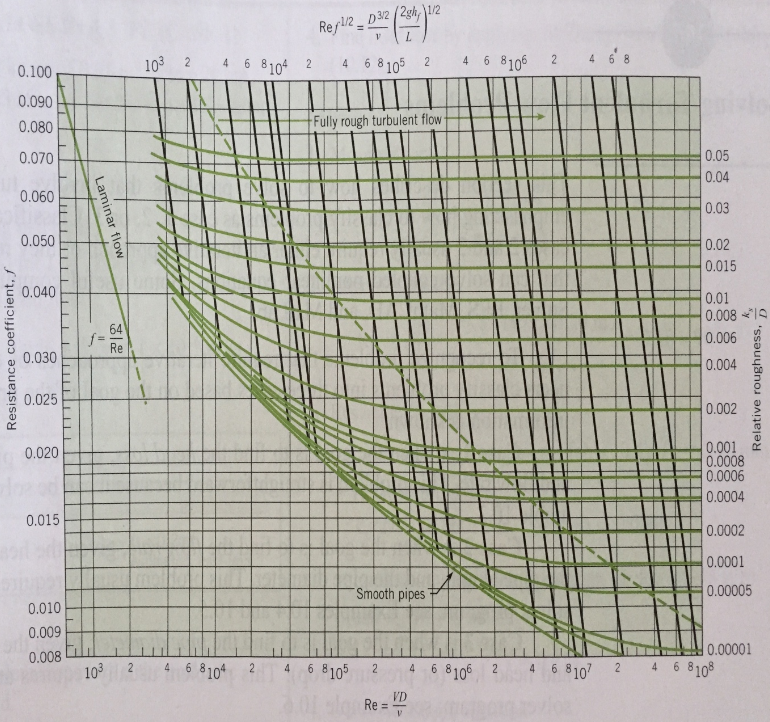
\includegraphics[scale=0.4128, angle = 90]{moodyDiagram.png}
    \caption{Moody Diagram}
    \label{fig:moodyDiagram}
\end{figure}



\end{document}